\chapter{Mercoledì 25/03/2020}
\section{Ciclo di vita}
Il progetto è un'attività essenziale nella realizzazione di un software. Si parte da una serie di esgienze e si arriva a una base di dati che le soddisfa. Tutte le attività svolte per arrivare all'oggetto desiderato vanno a formare il \textbf{ciclo di vita}.
\begin{definizione}[Ciclo di vita]
	Sequenza di attività, anche ripetute ciclicamente, svolte da analisti, progettisti, utenti, nello sviluppo e nell'uso dei sistemi software.
\end{definizione}
\noindent Le fasi tipiche del ciclo di vita sono:
\begin{itemize}
	\item \textbf{Raccolta e analisi dei requisiti}: si cerca di capire cosa bisogna fare, quali proprietà dovrà avere il software da progettare;
	\item \textbf{Progettazione}: individuazione delle funzionalità richieste dal sistema e dei dati necessari;
	\item \textbf{Realizzazione} vera e propria;
	\item \textbf{Collaudo}: sperimentazione, verifica che quanto progettato sia corretto;
	\item \textbf{Operatività}: il sistema diventa operativo.
\end{itemize}
\section{Concentriamoci sulla progettazione}
La progettazione riguarda sia i dati che le funzionalità del sistema. Nel caso dei sistemi informativi (questi) la parte fondamentale è quella riguardante la progettazione dei dati.
\paragraph{Buon progetto} Un buon progetto presenta un'adeguata documentazione di quanto fatto. Si usano dei modelli per rappresentare i dati in modo formale, preciso e comprensibile: utilizzo quindi dei linguaggi che permettano di seguire tutta la fase di progettazione e verificare durante il progetto il modo in cui i requisiti sono rispettati.
\paragraph{Modello per il ciclo di vita} Esistono moltissimi modelli, il più vecchio e utilizzato è il \emph{Waterfall model}. Le fasi di vita sono attraversate in sequenza una dopo l'altra. ogni volta che si passa a una fase viene chiusa la precedente e questa non viene più ripetuta.\\
Qualunque sia il modello adottato si hanno delle sottofasi:
\begin{itemize}
	\item \textbf{Acquisizione dei requisiti}: dipende molto dai rapporti umani tra cliente e sviluppatore. Si tiene conto anche di normative, regolamenti e procedure aziendali, realizzazioni già esistenti
	\item \textbf{Analisi dei requisiti}: presenti una serie di linguaggi necessari per definire i requisiti da più punti di vista
\end{itemize}
\paragraph{Come si acquisiscono i requisiti?} I requisiti possono essere acquisiti mediante documentazione (normative, regolamenti e procedure aziendali, realizzazioni già esistenti) e direttamente dall'utente. Questo aspetto è il più complesso nel processo di acquisizione: gli utenti potrebbero fornire informazioni diverse (chi sta in alto potrebbe avere visione più ampia, ma meno dettagliata). Segue la necessità, nel corso della progettazione, di parlare più volte con chi di dovuto \emph{raffinando} le informazioni già in nostro possesso.
\paragraph{Ranking dei requisiti} Nella fase di progettazione è necessario tenere conto del \emph{ranking} dei requisiti: alcuni sono più importanti di altri.
\paragraph{Quando siamo in possesso della documentazione necessaria?} La regola fondamentale è leggere ogni singola cosa in nostro possesso: una singola parola può fare la differenza! Raggruppiamo le frasi generali e le frasi relative ai vari concetti. Per chiarire il termine di concetto solitamente si inserisce nel progetto un \emph{Glossario} (per ciascun elemento si indica una descrizione, eventuali sinonimi e collegamenti).
\subsection{Esempio concreto degli ultimi passi spiegati}
\textit{Si vuole realizzare una base di dati per una società che eroga corsi: di ogni corso vogliamo rappresentare i dati dei partecipanti e dei docenti. Per gli studenti (circa 5000), identificati da un codice, si vuole memorizzare il codice fiscale, il cognome, l'età, il sesso, il luogo di nascita, il nome dei loro attuali datori di lavoro, i posti dove hanno lavorato in precedenza insieme al periodo, l'indirizzo e il numero di telefono, i corsi che hanno già frequentato (le materie sono in tutto circa 200) e il giudizio finale.}
\subsubsection{Glossario dei termini}
\begin{center}
	\begin{tabular}{ |l|l|l|l| } 
		\hline
		\textbf{Termine} & \textbf{Descrizione} & \textbf{Sinonimi} & \textbf{Collegamenti}\\
		\hline
		Partecipante & Persona che partecipa ai corsi & Studente & Corso, Società\\
		\hline
		Docente & Docenti dei corsi, che può essere esterno. & Insegnate & Corso\\
		\hline
		Corso & Corso organizzato dalla società. Può avere più edizioni. & Materia & Docente\\
		\hline
		Società & Ente presso cui i partecipanti lavorano o hanno lavorato & Posti & Partecipante\\
		\hline
	\end{tabular}
\end{center}
\subsubsection{Frasi di carattere generale}
\textit{Si vuole realizzare una base di dati per una società che eroga corsi: di ogni corso vogliamo rappresentare i dati dei partecipanti e dei docenti.}
\subsubsection{Frase relative ai partecipanti}
\textit{Per i partecipanti (circa 5000), identificati da un codice, rappresentiamo il codice fiscale, il cognome, l'età, il sesso, la città di nascita, i nomi dei loro attuali datori di lavoro e di quelli precedenti (insieme alle date di inizio e fine rapporto), le edizioni dei corsi che stanno attualmente frequentando e quelli che hanno frequentato nel passato, con la relativa votazione finale in decimi.}
\subsubsection{Frasi relative ai datori di lavoro}
\textit{Relativamente ai datori di lavoro presenti e passati dei partecipanti, rappresentiamo il nome, l'indirizzo e il numero di telefono.}
\subsubsection{Frasi relative ai corsi}
\textit{Per i corsi (circa 200), rappresentiamo il titolo e il codice, le varie edizioni con date di inizio e fine e, per ogni edizione, rappresentiamo il numero di partecipanti e il giorno della settimana, le aule e le ore dove sono tenute le lezioni.}
\subsubsection{Frasi relative a tipi specifici di partecipanti - sottoclassi di partecipanti a cui si vuole dare una rappresentazione particolare}
\textit{Per i partecipanti che sono liberi professionisti, rappresentiamo l'area di interesse e, se lo possiedono, il titolo professionale. Per i partecipanti che sono dipendenti, rappresentiamo invece il loro livello e la posizione ricoperta.}
\subsubsection{Frasi relative ai docenti}
\textit{Per i docenti (circa 300), rappresentiamo il cognome, l'età, la città di nascita, tutti i numeri di telefono, il titolo del corso che insegnano, di quelli che hanno insegnato nel passato e di quelli che possono insegnare. I docenti possono essere dipendenti interni della società di formazione o collaboratori esterni.}
\subsubsection{Morale della favola}
Non si inizia la progettazione finchè non si è letto tutto in modo adeguato.
\subsection{Progettazione per livelli di astrazione}
Si hanno vari livelli di astrazione per la progettazione:
\begin{itemize}
	\item \textbf{Livello concettuale}, il più esterno: esprime come deve essere fatto il sistema per rispettare i requisiti. Permette di vedere, nel nostro caso, l'organizzazione della base di dati
	\item \textbf{Livello logico}: si dice qualcosa sull'organizzazione dei dati. Le relazioni utilizzate, come sono collegate tra di loro...
	\item \textbf{Livello fisico}: vediamo dei blocchi in memoria secondaria. Si decide l'allocazione dei dati e le modalità di accesso nei momenti di lettura.\footnote{Un esempio di cosa da fare potrebbe essere uno studio sulle relazioni per valutare la creazione di uno o più indici, in modo tale da velocizzare le operazioni più frequenti}
\end{itemize}
Questi livelli di astrazione corrispondono a degli schemi in cui si usano modelli e linguaggi differenti per descrivere ciò che si rappresenta in ogni livello.
\begin{center}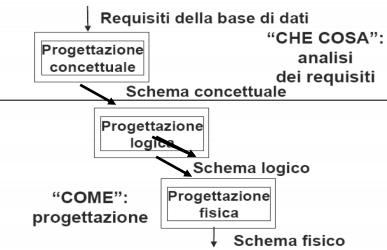
\includegraphics{images/3.PNG}\end{center}
\paragraph{Come si passa da un livello a un altro?} Facciamo una progettazione concettuale, li mettiamo nella rappresentazione, li verifichiamo e se tutto è valido compiamo un passaggio automatico da progettazione concettuale a progettazione logica. Se il progetto concettuale è ben fatto il progetto logico presenta esattamente le stesse proprietà. Il passaggio da progetto logico a fisico, invece, non è così automatico. Dopo la conclusione di una fase di progettazione si passa a quella successiva e non si ritorna più su quelle precedenti.
\subsection{Modelli concettuali}
Abbiamo bisogno di un buon linguaggio per descrivere lo schema concettuale. Abbiamo bisogno di un modello astratto il più vicino possibile all'essere umano: generalmente sono grafici semplici da usare e utili per interagire col cliente (quindi facilmente comprensibili anche da non-tecnici). I modelli esistenti sono formali (definiti in modo non ambiguo, descrivono in modo chiaro le caratteristiche di una base di dati) e integrati (descrivono tutte le caratteristiche della base di dati).
\begin{center}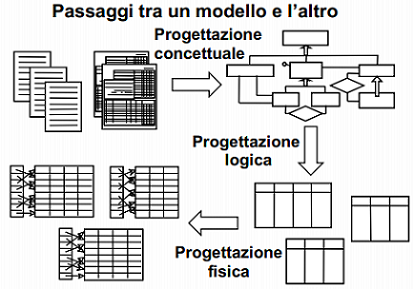
\includegraphics{images/4.PNG}\end{center}
\section{Modello E-R} Il modello più utilizzato è quello E-R (\emph{Entity-Relationship}): esso è il modello standard per descrivere una base di dati a livello concettuale.
\subsection{Costrutti del modello E-R}
Abbiamo tre costrutti di base: entità, relazioni e attributi. Si aggiungono i seguenti: identificatore e generalizzazione.
\subsubsection{Entita (\emph{entity})}
Un'entità è una classe di oggetti esistenti. Intendiamo fatti, persone, cose, impiegati, città, fatture, conti correnti... Ad ogni elemento sono associate delle proprietà comuni e con esistenza autonoma.\\

\noindent \textbf{Occorrenza di entità} Un'occorrenza è un elemento appartenente alla classe. A questo livello di progettazione so che un impiegato, per esempio, avrà certe proprietà: non mi interessa sapere i valori esatti ma so che possiede certe proprietà.\\
\textbf{Rappresentazione grafica} L'entità si rappresenta con un rettangolo avente un nome al suo interno.\begin{center}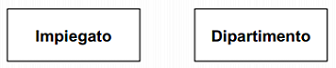
\includegraphics{images/5.PNG}\end{center}
\textbf{Convenzioni sui nomi} I nomi devono essere significativi (cioè che alludono in modo chiaro a cosa intendiamo) e possibilmente singolari.
\subsubsection{Associazioni (\emph{relationship})}
L'associazione è un legame fra due o più entità. Prendiamo per esempio studenti, esami e insegnamenti. Lo studente svolge un esame per un certo corso!	\\	

\noindent \textbf{Rappresentazione grafica} Le associazioni si rappresentano mediante rombi con all'interno il nome dell'associazione. Il rombo è collegato alle due entità collegate. Si osserva che non sono presenti frecce: non si ha un verso, chi viene prima e chi viene dopo non ha importanza.\begin{center}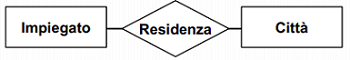
\includegraphics{images/6.PNG}\end{center}
\textbf{Convenzioni sui nomi} Anche qui i nomi devono essere espressivi e singolari. Importante usare sostantivi e non verbi: il verbo attribuisce un verso all'associazione e abbiamo detto che non ci sono frecce.\\
\textbf{Occorrenza di associazione} Un insieme di tuple, di occorrenze di entità. Se l'associazione è fra $t$ entità avrò $t$ tuple, ciascuna per ogni entità coinvolta. Non posso avere occorrenze ripetute, se ne ha una sola. L'occorrenza è definita come una coppia.
\paragraph{Domanda}
Questa base di dati consisterà in una rappresentazione del libretto elettronico o in un supporto a statini per la creazione di statistiche? Un uso diverso può comportare una progettazione diversa.
\begin{itemize}
	\item Se voglio realizzare semplicemente un libretto elettronico mi limito a indicare l'esame passato con la data e la valutazione
	\item Se voglio fare un supporto a statini allora ho bisogno di ulteriori informazioni: non soltanto l'ultimo esame passato ma anche i tentativi. Se progetto una base di dati come un libretto elettronico non posso trovare queste informazioni! Si deve organizzare la base di dati in modo che queste operazioni siano realizzabili: includeremo a tal proposito una nuova entità \emph{DataEsame}.
\end{itemize}
\paragraph{Passaggio da una rappresentazione per libretto a rappresentazione per supporto a statini}
\begin{center}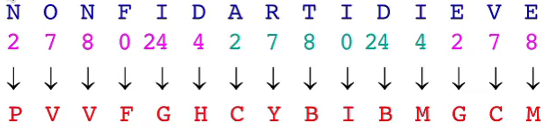
\includegraphics{images/9.PNG}\end{center}

\paragraph{Relationship diverse sulle stesse entità} Possono esistere più relazioni tra le stesse entità. L'impiegato può essere associato, per esempio, a due città: quella di residenza e quella di lavoro. Le due città possono coincidere ma possono essere anche diverse!
\begin{center}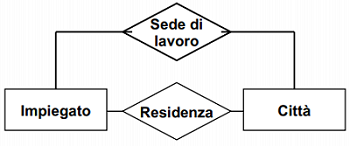
\includegraphics{images/10.PNG}\end{center}
\paragraph{Relationship ricorsiva} Un'entità può comparire più volte nell'associazione. Lego una persona, per esempio, a un'altra persona: ho l'occorrenza conoscenza che riguarda due persone che si conoscono. Posso stabilire, in alcuni casi, ruoli nella relazione ricorsiva: ho l'entità sovrano e la relazione successione, dove distinguo successore da predecessore.
\begin{center}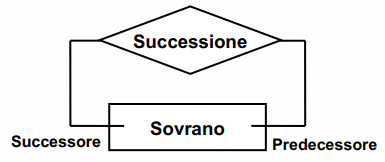
\includegraphics{images/11.PNG}\end{center}
\paragraph{Relationship mista} Posso mescolare ricorsione con ricorsione.

\subsubsection{Attributo}
Proprietà elementare di un'entità o di un'associazione.  L'attributo ha un certo dominio (o stringa, o intero, o data...) e il valore è associato ad occorrenze di entità o associazione.\\

\noindent \textbf{Rappresentazione grafica} Gli attributi si rappresentano attraverso grafi.
\begin{center}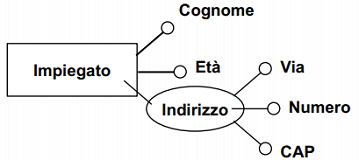
\includegraphics{images/12.PNG}\end{center}
Risulta possibile strutturare gli attributi in modo più dettagliato. Posso raggruppare parte degli attributi in un unico gruppo. La cosa è soprattutto grafica! Il nome dell'attributo composto è racchiuso all'interno di un "cerchio schiacciato".

\subsection{Esempio concreto}
\paragraph{Testo} \textit{Si vuole descrivere l'organizzazione di un'azienda
	\begin{itemize}
		\item Con sedi diverse
		\item Ogni sede è composta di vari dipartimenti
		\item Gli impiegati dell'azienda afferiscono ai vari dipartimenti e un'impiegato li dirige
		\item Gli impiegati lavorano su progetti
		\item Ogni entità o relationship può avere vari attributi
\end{itemize}}
\paragraph{Immagine} \begin{center}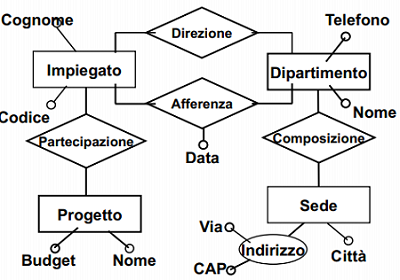
\includegraphics{images/17.PNG}\end{center}
\begin{itemize}
	\item Le entità presenti (concrete) sono Impiegato, Dipartimento, Progetto e Sede.
	\item Individuo gli attributi che descrivono le varie entità.
	\item Gli impiegati lavorano sui progetti, quindi stabilisco una relazione tra impiegato e progetto.
	\item L'impiegato afferisce a un dipartimento, cioè può decidere in quale dipartimento stare. Uno degli impiegati, inoltre, dirige un dipartimento
	\item In ogni sede ci sono più dipartimenti, ogni dipartimento ha una sede in cui è collocato.
\end{itemize}
\paragraph{Torno dal cliente e gli faccio vedere lo schema} Il cliente muove delle osservazioni, dettagli nuovi da aggiungere:
\begin{itemize}
	\item un dipartimento ha un solo direttore
	\item un impiegato può afferire ad un solo dipartimento
	\item il direttore di dipartimento afferisce a quel dipartimento
\end{itemize}
Lo schema è incompleto e non possiamo aggiungere i dettagli richiesti utilizzando solo i costrutti base.

\subsection{Cardinalità}
La cardinalità mi permette di stabilire, per esempio, quante coppie posso stabilire in un'associazione. Generalmente consiste in una coppia di valori associati a ogni entità che partecipa a una relazione: specifica il numero minimo e massimo di occorrenze della relazione cui ciascuna occorrenza di entità può partecipare.\\

\noindent \textbf{Rappresentazione grafica} La cardinalità si rappresenta etichettando le entità.\\
\textbf{Simbologia} I simboli adottabili nella cardinalità sono
\begin{itemize}
	\item numeri, ponibili sia nella cardinalità minima che in quella massima
	\item $N$, ponibile solo nella cardinalità massima, che attesta un numero formalmente illimitato di associazioni.
\end{itemize}
\textbf{Esempio grafico} \begin{center}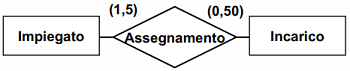
\includegraphics{images/14.PNG}\end{center}
\begin{itemize}
	\item Ogni impiegato ha un incarico ma non ne può avere più di cinque
	\item L'incarico può essere assegnato a un massimo di cinquanta persone, ma può essere anche non assegnato.
\end{itemize}
\textbf{Esempio grafico 2} \begin{center}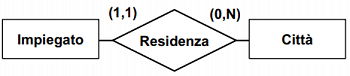
\includegraphics{images/15.PNG}\end{center}
\begin{itemize}
	\item L'impiegato è associato a una e una sola città di residenza
	\item La città può essere associata a un numero infinito di impiegati, ma può essere anche priva di relazioni con gli impiegati
\end{itemize}
\textbf{Tipi di relationship} Attraverso le cardinalità massime possiamo definire i seguenti tipi di relationship:
\begin{itemize}
	\item uno a uno (la cardinalità massima è sempre $1$)
	\begin{center}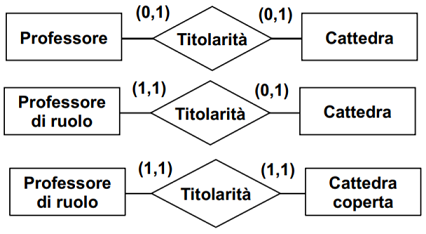
\includegraphics{images/149.PNG}\end{center}
	\item uno a molti (una delle due cardinalità massime è $1$, l'altra $N$)
	\begin{center}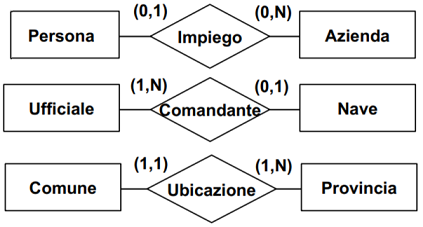
\includegraphics{images/147.PNG}\end{center}
	\item molti a molti (entrambe le cardinalità massime sono $N$)
	\begin{center}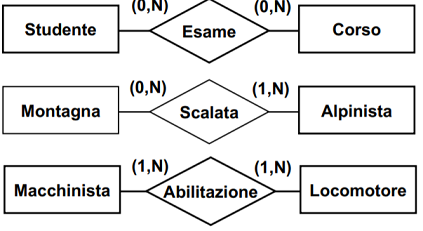
\includegraphics{images/148.PNG}\end{center}
\end{itemize}
\textbf{Cardinalità di attributi} Posso associare cardinalità anche agli attributi per indicare opzionalità dell'informazione o attributi multivalore.
\clearpage
\paragraph{Esempio cardinalità di attributi} \begin{center}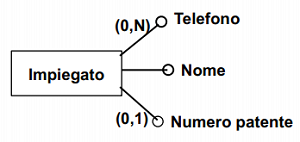
\includegraphics{images/16.PNG}\end{center}
\begin{itemize}
	\item L'impiegato può essere associato a un numero infinito di telefoni (non solo quello personale, ma anche quello aziendale...) o a nessun telefono
	\item L'impiegato può essere privo di patente o avere una sola patente.
\end{itemize}
\subsection{Riprendiamo lo schema E-R dell'azienda e poniamo le cardinalità}
\begin{center}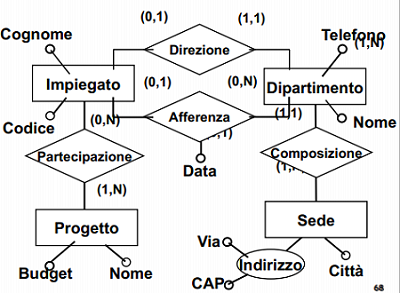
\includegraphics{images/18.PNG}\end{center}
\begin{itemize}
	\item Il dipartimento ha uno e un solo direttore (c'è sempre, quando aggiungo un nuovo dipartimento conosco già il direttore). L'impiegato può essere direttore ma può anche non esserlo
	\item Il dipartimento può essere privo di afferenze ma ne può avere un numero illimitato. L'impiegato può non avere afferenza, ma ne ha al massimo una (quindi l'impiegato può decidere di porsi in un certo dipartimento anche dopo l'assunzione). Segue che la data di afferenza può essere assente, e che ce ne sia al massimo una.
	\item Il dipartimento può avere infiniti numeri di telefono, ma almeno uno.
	\item L'impiegato può essere assegnato a un numero infinito di progetti, ma potrebbe anche essere privo di incarichi. Un progetto deve avere almeno un impiegato incaricato (ovviamente non si hanno limiti nel numero di persone assegnabili a un progetto).
	\item Il dipartimento sta in una sola sede. La sede ha almeno un dipartimento, ma può ospitare più di un dipartimento
\end{itemize}
\paragraph{Ritorno nuovamente dal cliente} I primi due dettagli sono sistemati, l'ultimo (quello di afferenza del direttore di dipartimento) no! Per il controllo di questa cosa, basato su valori, dobbiamo aggiungere la data di inizio direzione in modo da poter verificare che il direttore abbia assunto l'incarico dopo aver afferito a un certo dipartimento.

\subsection{Identificatore di un'entità}
Con le cardinalità si impongono vincoli generali sulle occorrenze delle associazioni. La scelta dell'identificatore permette di arricchire ulteriormente lo schema: ne può avere più di uno, ma ne deve avere per forza uno.\\L'identificatore può essere, per esempio, la targa di un automobile (se abbiamo un'entità Automobile) o tre attributi (Cognome, Nome e DataNascita) per l'entità Persona.\\

\noindent \textbf{Identificatori esterni}: ho una base di dati con gli studenti di tutta Italia. Uno studente di un certo ateneo è identificato da una matricola: tuttavia potrei avere uno studente, in un altro ateneo, avente la stessa matricola. Quindi devo utilizzare come identificatore non solo la matricola, ma anche il nome dell'università: questo identificatore lo devo prendere da un'altra tabella per evitare che vengano inseriti atenei inesistenti (Per esempio l'\emph{ateneo di Fornacette}). Segue l'uso di un vincolo di integrità referenziale.\\
L'identificatore esterno può essere utilizzato solo con cardinalità $(1,1)$: se avessi uno studente iscritto a più università in Italia quanto detto non funzionerebbe.
\begin{center}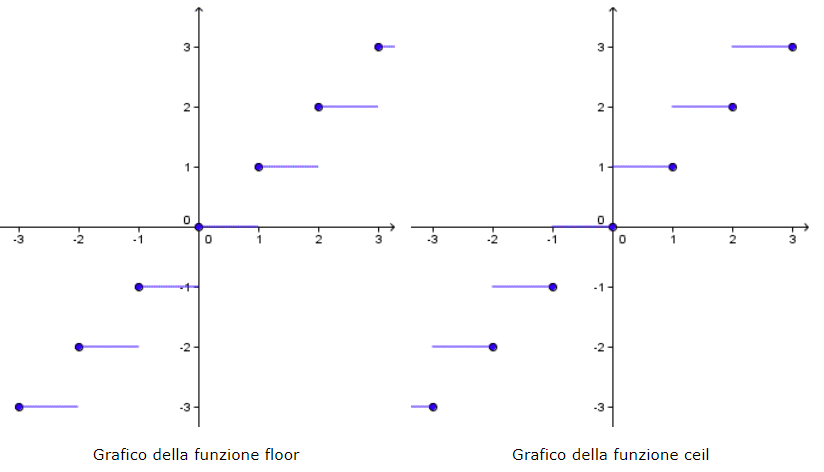
\includegraphics{images/19.PNG}\end{center}

\subsection{Mettiamo gli identificatori nello schema E-R}
\begin{center}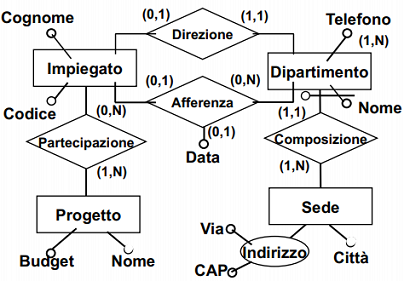
\includegraphics{images/20.PNG}\end{center}
\begin{itemize}
	\item Ogni impiegato ha un codice univoco identificativo
	\item Ogni progetto è identificato dal nome
	\item La sede è identificata dalla città (quindi una sola sede per città)
	\item Il dipartimento è identificato dal nome e dalla città (identificatore esterno)
\end{itemize}
Nelle associazioni non ho identificatori poichè l'identificatore è costituito dalla coppia associata.
\subsection{Generalizzazione}
La generalizzazione è un costrutto utile quando si stabilisce il modello concettuale ma che viene perso col passaggio ai modelli successivi. Si ha un concetto gerarchico. Ho l'entità Dipendente, posso stabilire l'esistenza di sue sottoclassi: impiegato, funzionario e dirigente. Sono distinti da attributi specifici che rendono diversa una sottoclasse dall'altra (lo stipendio, la residenza...).
\begin{center}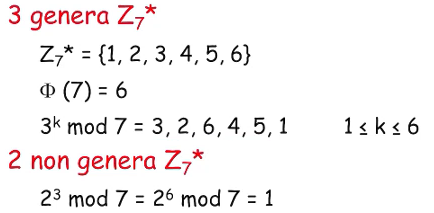
\includegraphics{images/23.PNG}\end{center}
Tutte le proprietà dell'entità genitore vengono ereditate dalle figlie e non rappresentate esplicitamente.\\
\textbf{Tipi di generalizzazione} La generalizzazione può essere
\begin{itemize}
	\item \textbf{Totale}: freccia piena, se ogni occorrenza dell'entità genitore è occorrenza di almeno una delle entità figlie (Esempio: le occorrenze di persona sono uomini o donne, nient'altro).
	\item \textbf{Parziale}: freccia vuota, esistono occorrenze dell'entità genitore che non sono occorrenze di entità figlie (Esempio: esistono occorrenze di persona che non sono nè studenti nè lavoratori).
\end{itemize}
La generalizzazione si dice:
\begin{itemize}
	\item \textbf{Esclusiva}: se ogni occorrenza dell'entità genitore è occorrenza di al più una delle entità figlie (Esempio: gli studenti lavoratori sono persone ma esistono occorrenze di persona che non sono ne studenti nè lavoratori).
	\item \textbf{Sovrapposta}: esistono occorrenze dell'entità genitore che sono occorrenze di più di una delle entità figlie (Esempio: ho uno studente lavoratore, un'occorrenza dell'entità persona è occorrenza sia di studente che di lavoratore).
\end{itemize}
\textbf{Gerarchia con una sottoclasse} Posso avere una gerarchia con una sola sottoclasse. Segue che avrò una generalizzazione di tipo parziale: è ovvio che se pongo solo una sottoclasse allora esisteranno occorrenze dell'entità genitore che non sono occorrenze dell'entità figlia (altrimenti farei prima a togliere il costruttore chiamando l'entità genitore come l'entità figlia).\\
\textbf{Alberi paralleli di gerarchia} Sono possibili alberi di gerarchia parallela, cioè fare partire più alberi dall'entità genitore. In questi alberi si distingue generalizzazione di tipo totale da generalizzazione di tipo parziale.
\begin{center}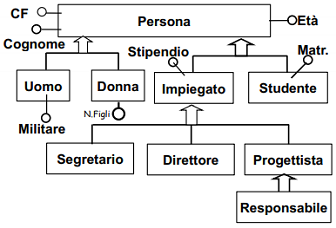
\includegraphics{images/22.PNG}\end{center}
\subsection{Documentazione associata agli schemi E-R}
\begin{center}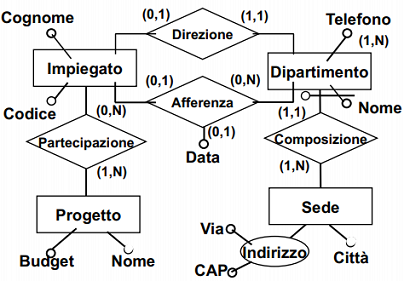
\includegraphics{images/20.PNG}\end{center}
Lo schema e basta non è mai sufficiente per rappresentare tutti i dettagli di un'applicazione. Ci sono vincoli non esprimibili (Esempio: il direttore che afferisce al dipartimento che dirige). Si pone in forma cartacea ciò che non è visibile dal grafico e anche ciò che lo è.
\subsubsection*{Dizionari dei dati (entità)} 
\begin{center}
	\begin{tabular}{ |l|l|l|l| } 
		\hline
		\textbf{Entità} & \textbf{Descrizione} & \textbf{Attributi} & \textbf{Identificatore}\\
		\hline
		Impiegato & Dipendente dell'azienda & Codice, Cognome & Codice\\
		\hline
		Progetto & Progetti aziendali & Nome, Budget & Nome\\
		\hline
		Dipartimento & Struttura aziendale & Nome, Telefono & Nome, Sede\\
		\hline
		Sede & Sede dell'azienda & Città, Indirizzo & Città\\
		\hline
	\end{tabular}
\end{center}
\subsubsection*{Dizionari dei dati (relationship)} 
\begin{center}
	\begin{tabular}{ |l|l|l|l| } 
		\hline
		\textbf{Relazioni} & \textbf{Descrizione} & \textbf{Componenti} & \textbf{Attributi}\\
		\hline
		Direzion & Direzione di un dipartimento & Impiegato, Dipartimento & \\
		\hline
		Afferenza & Afferenza a un dipartimento & Impiegato, Dipartimento & Data\\
		\hline
		Partecipazione & Partecipazione a un progetto & Impiegato, Progetto & \\
		\hline
		Composizione & Composizione dell'azienda & Dipartimento, Sede & \\
		\hline
	\end{tabular}
\end{center}
\subsubsection*{Regole di vincolo}
\begin{enumerate}
	\item Il direttore di un dipartimento deve afferire a tale dipartimento
	\item Un impiegato non deve avere uno stipendio maggiore del diretto del dipartimento al quale afferisce
	\item Un dipartimento con sede a Roma deve essere diretto da un impiegato con più di dieci anni di anzianità
	\item Un impiegato che non afferisce a nessun dipartimento non deve partecipare a nessun progetto
\end{enumerate}
\subsubsection*{Regole di derivazione}
\begin{enumerate}
	\item Il numero di impiegati di un dipartimento si ottiene contando gli impiegati che afferiscono a tale dipartimento
	\item Il budget di un progetto si ottiene moltiplicando per 3 la somma degli stipendi degli impiegati che vi partecipano
\end{enumerate}


\noindent I vincoli espressi in precedenza e le regole di derivazione riguardano i valori che vengono immessi nelle entità e associazioni in esecuzione.
\subsection{Quali costrutti scelgo?}
Per la scelta dei costrutti mi baso sulle loro definizioni
\begin{itemize}
	\item \textbf{Entità}: Se ha proprietà significativa e descrive oggetti con esistenza autonoma
	\item \textbf{Attributo}: Se è semplice e non ha proprietà
	\item \textbf{Associazione}: Se correla due o più concetti
	\item \textbf{Generalizzazione}: Se è caso particolare di un altro
\end{itemize}
\subsection{Quali caratteristiche deve avere il mio schema?}
Uno schema deve essere
\begin{multicols}{4}
	\begin{itemize}
		\item Corretto
		\item Completo 
		\item Leggibile
		\item Minimale 
	\end{itemize}
\end{multicols}
\subsection{Strategie di progetto}
\begin{itemize}
	\item \textbf{top-down}: parto da uno schema iniziale, lo raffino e integro mediante primitive che lo trasformano in una serie di schemi intermedi. Collego questi schemi e arrivo allo schema E-R finale. Le primitive di raffinamento sono:
	\begin{itemize}
		\item Da entità ad associazione tra entità
		\item Da entità a generalizzazione
		\item Da associazione a insiemi di associazioni
		\item Da associazione a entità con associazioni
		\item Introduzione di attributi su entità e associazioni
	\end{itemize}
	\item \textbf{bottom-up}: al contrario. Parto da specifiche iniziali, le divido fino a ottenere una specifica componente minima da cui nasce lo schema E-R. Gli schemi prodotti vengono fusi e integrati fino ad ottenere lo schema finale. Le primitive sono:
	\begin{itemize}
		\item Generazione di entità
		\item Generazione di associazione
		\item Generazione di generalizzazione
	\end{itemize}
\end{itemize}
Solitamente la strategia adottata è mista:
\begin{itemize}
	\item inizialmente individuo i concetti principali realizzando uno schema scheletro
	\item lo decompongo se necessario
	\item poi lo raffino, espando ed integro.
\end{itemize}
\paragraph{Definizione dello schema scheletro} Schema che contiene i concetti più importanti, i più citati o indicati esplicitamente come cruciali.
